\chapter{从函数拟合到概率分布}
\label{chap:probability-language}

\begin{keybox}[从拟合函数到拟合分布]
监督学习拟合的是一条从输入到答案的映射；生成模型要拟合的是对象空间上的整个分布。这一章先把这条跳跃拆开：损失函数在优化什么、梯度怎样沿计算图传回、判别与生成分别回答哪个条件概率、以及怎样比较两个分布。KL 的方向和变分自由能会在这里第一次出现，后面判断一个模型是覆盖所有模式还是只抓住一个，都要回到这两个量。
\end{keybox}

\section{一条训练链：从样本到参数更新}

\subsection{分类、拟合与损失函数}

先看最普通的监督学习。数据集 \(\mathcal D=\{(x_i,y_i)\}_{i=1}^N\) 给出输入及其已知答案；例如 \(x_i\) 可以是一个自旋构型，\(y_i\) 是相标签或能量。\textbf{分类}要求预测有限个类别：二分类时 \(y_i\in\{0,1\}\)，模型可输出属于第 1 类的概率 \(q_\theta(x_i)\in(0,1)\)，再用阈值作出类别判断。若答案是连续的能量数值，任务则是回归。两者都先选择一个带可调参数 \(\theta\) 的函数 \(f_\theta(x)\)，再用数据决定参数的取值；这就是函数的\textbf{参数化}与\textbf{拟合}。参数可以是线性模型的系数，也可以是神经网络各层的权重和偏置。

拟合需要把预测好坏化成可计算的标量。逐样本损失 \(\ell\) 衡量预测与答案的差异，经验损失是数据集上的平均：
\begin{equation}
  L(\theta)=\frac{1}{N}\sum_{i=1}^N \ell\bigl(f_\theta(x_i),y_i\bigr).
  \label{eq:basic-empirical-loss}
\end{equation}
对连续目标，常用均方误差（Mean Squared Error，MSE）对应的逐样本平方损失 \(\ell_{\mathrm{MSE}}=(f_\theta(x)-y)^2\)；对二分类概率，常用交叉熵（Cross-Entropy，CE）
\begin{equation}
  \ell_{\mathrm{CE}}=-y\log q_\theta(x)-(1-y)\log\bigl(1-q_\theta(x)\bigr).
  \label{eq:basic-binary-ce}
\end{equation}
预测的正确类别概率越小，交叉熵越大；多分类时相应地在所有类别上输出归一化概率，并取真实类别概率的负对数。损失函数说明\textbf{训练时优化什么}，分类正确率等评价量则说明\textbf{最终怎样衡量表现}，两者可以不同。训练集上的低损失只说明已见样本拟合得好，还需要用未参与参数更新的验证或测试数据检查泛化。

\subsection{梯度下降与自动微分}

当 \(L(\theta)\) 对参数可微时，梯度 \(\nabla_\theta L\) 给出每个参数微小变化对损失的一阶影响。最简单的梯度下降更新为
\begin{equation}
  \theta_{k+1}=\theta_k-\eta\nabla_\theta L(\theta_k),
  \label{eq:basic-gradient-descent}
\end{equation}
其中 \(\eta>0\) 是学习率；实际训练常用随机抽取的一小批样本估计梯度，并使用自适应优化器。优化是反复计算预测、损失和梯度，再更新参数的过程。梯度下降寻找的是当前参数附近的下降方向，不保证在非凸问题中找到全局最优，也不能单独保证泛化。

自动微分把实际执行的计算拆成加法、矩阵乘法、激活函数等基本运算，记录它们构成的计算图，再按链式法则求导。训练神经网络通常使用反向模式：先前向得到损失标量，再从损失沿计算图反向累积 \(\partial L/\partial\theta\)，这就是反向传播。自动微分负责计算梯度，梯度下降或 Adam 等优化器负责利用梯度改变参数；它们是训练链中的两个不同步骤。自动微分沿计算图求得程序中各可微运算的导数；遇到离散抽样等不可直接求导的步骤，还需要另外设计梯度估计方法。

\section{为什么神经网络适合表示函数}

多层感知机（Multilayer Perceptron，MLP）是最基本的前馈神经网络。一个含单个隐藏层的例子是
\begin{equation}
  f_\theta(x)=W_2\,\sigma(W_1x+b_1)+b_2,
  \qquad \theta=(W_1,b_1,W_2,b_2),
  \label{eq:basic-mlp}
\end{equation}
其中矩阵乘法混合输入分量，非线性激活 \(\sigma\) 让模型能表达弯曲的决策边界或非线性响应；若去掉激活，多层仿射变换仍只是一个仿射变换。增加层数就是反复组合这两种操作。用于二分类时，可把标量输出当作 logit，经 sigmoid 函数 \(q_\theta(x)=1/(1+e^{-f_\theta(x)})\) 变成概率；用于回归时，可以直接输出数值。网络的特征变换由数据共同学习，参数可沿计算图求梯度，矩阵运算也适合批量计算。图像、序列等结构化输入通常需要卷积、注意力等进一步的结构设计，后文的 Transformer 就是一种例子。

\textbf{通用近似定理}给出表达能力的一个边界：对紧致区域上的连续函数，在合适的非线性激活条件下，单隐藏层网络只要有足够多的隐藏单元，就能把函数逼近到任意指定的精度~\cite{cybenko1989approximation,hornik1991approximation}。这是一个\textbf{存在性}结论，描述表达能力的上限；实际能否学到还取决于样本量、优化和归纳偏置。神经网络实用的原因还包括可学习的组合特征、可扩展的计算以及对任务结构的适配。接下来把网络输出从数值或类别概率推广到整个数据分布，就进入生成模型的问题。

\section{判别、生成与逆向设计}

判别模型通常直接学习 \(p(y\mid x)\) 或一个决策函数，目标是给定观测 \(x\) 预测标签 \(y\)。生成模型试图刻画 \(p(x)\)，或者在给定条件 \(c\) 后刻画 \(p(x\mid c)\)，从而可以生成新的样本、补全缺失变量、估计似然或做逆向设计（图 \ref{fig:discriminative-generative}）。

\begin{figure}[ht]
\centering
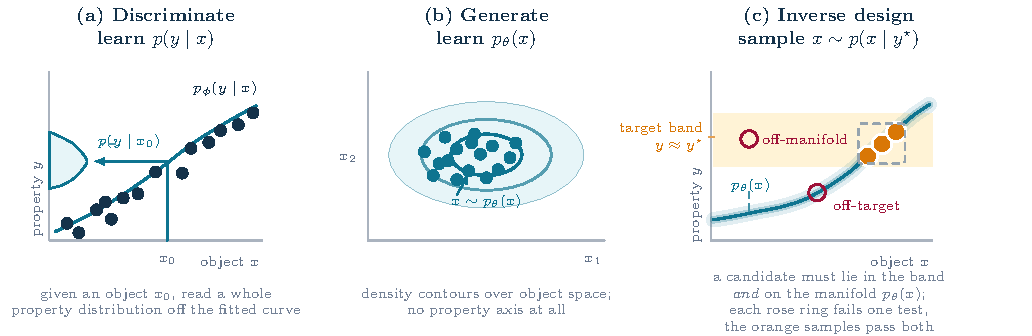
\includegraphics[width=\textwidth]{discriminate_generate_inverse.pdf}
\caption{三个任务使用同一批对象，却回答不同问题：判别模型沿已知对象预测性质；生成模型学习对象空间的概率质量；逆向设计只在目标性质带内寻找仍位于合理数据分布上的候选。}
\label{fig:discriminative-generative}
\end{figure}

贝叶斯公式（Bayes' rule）把这两个方向连接起来：
\begin{equation}
  p(x\mid y)=\frac{p(y\mid x)p(x)}{p(y)}\propto p(y\mid x)p(x).
\end{equation}
这条公式把生成问题中的三个概率对象连接起来，是一段纯粹的恒等变形，不需要任何神经网络参与。设 \(x\) 是待生成的候选结构、分子、图像或文本，\(y\) 是由它产生的观测、类别或目标性质。\(p(x)\) 是先验或无条件生成分布，表示什么样的 \(x\) 在数据中本来就合理；\(p(y\mid x)\) 是正向模型或似然，表示给定候选 \(x\) 后观察到目标 \(y\) 的概率；\(p(x\mid y)\) 是逆向问题真正需要的后验，表示在满足目标 \(y\) 的候选中，哪些 \(x\) 仍然符合数据分布。

例如，设 \(x\) 是候选分子，\(y^\star\) 是目标带隙。训练好的生成模型 \(p_\theta(x)\) 描述哪些分子通常合理，性质预测器 \(p_\phi(y^\star\mid x)\) 描述这些分子满足目标的程度，两者的乘积给出后验的相对权重。如果任务只需要一个候选，可以固定模型参数、对 \(x\) 最大化这个乘积；如果希望保留多个可行结构及其不确定性，就应从后验中采样。仅最大化性质预测器的输出，可能选到训练分布之外的畸形分子；加入先验后，候选还需要得到结构分布的支持。

实现条件生成有两条路线（图 \ref{fig:bayes-generative-models}），区别在于条件分布从哪里来。\textbf{先建模再推断}：分别得到 \(p_\theta(x)\) 与 \(p_\phi(y\mid x)\)，对给定的 \(y\) 用贝叶斯公式构造后验。\textbf{直接学习条件分布}：用配对数据 \((x,y)\) 训练一个条件生成器 \(p_\psi(x\mid y)\)，让同一个网络能够处理不同的 \(y\)。例如，条件自回归模型把 \(y\) 放入每一步生成的条件，条件扩散模型把 \(y\) 送入去噪网络；具体采样过程在第 \ref{chap:model-families} 章展开。

两条路线都必须得到归一化的输出分布，但无需用同一种方式计算归一化因子。先建模再推断时，设 \(\widetilde p_y(x)=p_\theta(x)p_\phi(y\mid x)\)，后验为 \(p(x\mid y)=\widetilde p_y(x)/Z_y\)，其中 \(Z_y=\int\widetilde p_y(x)\,dx\) 通常难算。直接学习条件分布时，归一化由模型构造保证，例如自回归模型的每个条件概率都在词表上归一化，扩散模型由归一化的反向转移逐步采样。这条路线需要足够的配对数据，并承担模型近似和训练误差；它不需要额外计算上述乘积模型的 \(Z_y\)。

回到上面的分子例子，用三个候选把这一步算出来。设它们的先验为 \(p(x_A),p(x_B),p(x_C)=(0.5,0.3,0.2)\)，性质预测器给出 \(p(y^\star\mid x)=(0.1,0.6,0.4)\)。把两项相乘再做归一化，就得到每个候选在后验中的权重（表 \ref{tab:inverse-design-weights}）。

\begin{table}[H]
\centering\small
\begin{tabularx}{\textwidth}{>{\bfseries}p{16mm} X X X X}
\toprule
候选 & 先验 \(p(x)\) & 性质似然 \(p(y^\star\mid x)\) & 乘积 \(\widetilde p_y(x)\) & 归一化后验\\
\midrule
A & 0.5 & 0.1 & 0.05 & 0.16\\
B & 0.3 & 0.6 & 0.18 & 0.58\\
C & 0.2 & 0.4 & 0.08 & 0.26\\
\bottomrule
\end{tabularx}
\caption{三个候选的逆向设计权重。\(Z_{y^\star}=0.05+0.18+0.08=0.31\)。}
\label{tab:inverse-design-weights}
\end{table}

候选 B 的性质最匹配，但先验只有 0.3；候选 A 先验最高，性质却不匹配；C 两项都不突出，后验居中。若只按性质预测器排序，B 仍然第一，但当两个候选的性质分数接近时，先验会改变排序——这正是逆向设计里加入 \(p(x)\) 的作用。

对于已经由 \(\widetilde p_y\) 给出的后验，下面两种方法分别通过采样和优化处理难算的 \(Z_y\)。马尔可夫链蒙特卡洛（Markov Chain Monte Carlo，MCMC）设计转移核 \(K(x'\mid x)\)，使目标后验成为平稳分布，即
\begin{equation}
 p(x'\mid y)=\int K(x'\mid x)p(x\mid y)\,dx.
\end{equation}
接受率可以只依赖 \(\widetilde p_y(x')/\widetilde p_y(x)\)，从而约掉 \(Z_y\)。在链具有遍历性等收敛条件、运行足够久且能跨越不同高概率区域时，样本的经验分布才逼近目标后验；通常丢弃一段初始过渡期（burn-in），并检查样本相关性与跨模式移动。

变分推断（Variational Inference，VI）选择一个归一化、可采样且可求密度的分布族 \(q_\varphi(x)\)，通过优化让它接近后验。这里用 Kullback--Leibler 散度（Kullback--Leibler divergence，KL）衡量两个分布的差异，其定义及在本问题中的展开为
\begin{align}
 \KL(q\Vert p)&=\int q(x)\log\frac{q(x)}{p(x)}\,dx,\\
 \KL(q_\varphi\Vert p(\cdot\mid y))
 &=\E_{q_\varphi}\!\left[\log q_\varphi(x)-\log\widetilde p_y(x)\right]+\log Z_y.
 \label{eq:vi-normalizer}
\end{align}
固定先验、性质预测器和条件 \(y\) 后，\(Z_y\) 与变分参数 \(\varphi\) 无关。因此最小化第一项就能找到同一个最优 \(q_\varphi\)，虽然无法由此报告 KL 的绝对数值。优化完成后，从 \(q_\varphi\) 采样的代价通常较低，误差来自所选分布族和优化结果。若同时改变 \(\theta\) 或 \(\phi\)，\(Z_y\) 一般也会变化，就不能在这些参数的梯度中直接忽略它。

MCMC 与 VI 都可用于“先建模再推断”路线中的后验计算。前者逐步更新样本，后者先拟合近似后验；直接从配对数据训练条件生成器是前面另一层面的建模选择，也可以使用变分训练。这两个层面的选择共同决定需要什么数据、优化什么目标以及最终如何取样。

\begin{figure}[H]
\centering
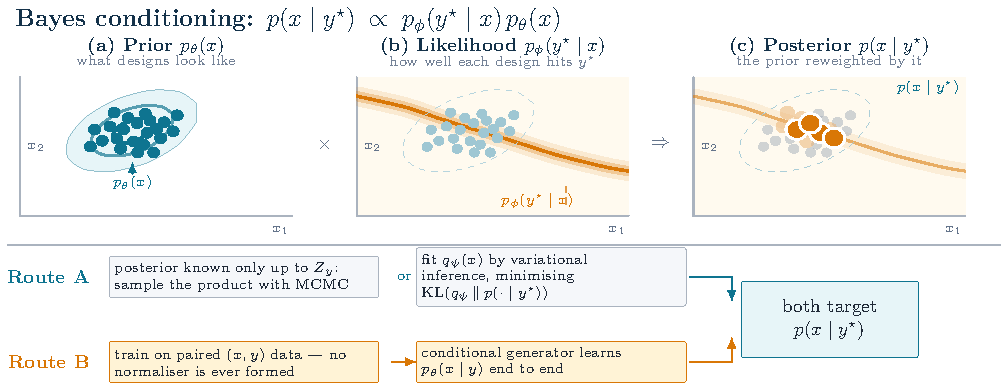
\includegraphics[width=\textwidth]{bayes_conditioning.pdf}
\caption{条件生成的两条建模路线。上方示意先验经目标性质的似然重新加权；路线 A 在给定乘积后验上使用 MCMC 或 VI，路线 B 从配对数据学习条件生成器。两者可以指向同一目标条件分布，有限数据、近似推断和模型误差决定实际差异。}
\label{fig:bayes-generative-models}
\end{figure}

\section{KL 方向与统计物理中的自由能}

\subsection{KL 的方向与模式覆盖}

上一节的 VI 需要选择分布间的差异度量。KL 非负，但带有方向。记 \(p\) 为目标分布（例如数据分布），\(q\) 为模型，则 \(\KL(p\Vert q)\neq\KL(q\Vert p)\)。前者在目标分布上取期望，若某个模式真实出现却被模型赋予极小概率，惩罚会很大，这一方向因此要求模型覆盖数据的全部模式；后者在模型自己的样本上取期望，更关心模型生成的样本是否进入目标分布的高概率区域。同一个散度写在哪一侧，决定了哪些区域的误差被赋予更大权重。

图 \ref{fig:kl-direction} 用单个高斯 \(q\) 拟合等权双峰目标 \(p\)。前向 \(\KL(p\Vert q)\) 在 \(p\) 下取期望，对高斯族的最优解恰好匹配 \(p\) 的均值与方差，于是 \(q\) 横跨两峰，也把质量放进了两峰之间的低谷。反向 \(\KL(q\Vert p)\) 在 \(q\) 下取期望，\(q\) 在 \(p\approx0\) 处的质量受到 \(\log(q/p)\) 的重罚，它只好躲进一个峰，另一个峰被整个丢掉。后文反复回到这两种行为：最大似然训练的模型倾向于覆盖所有模式，样本可能落在模式之间；生成对抗网络（Generative Adversarial Network，GAN）的模式坍缩、后训练中的分布坍缩则更接近反向 KL 的行为。

\begin{figure}[H]
\centering
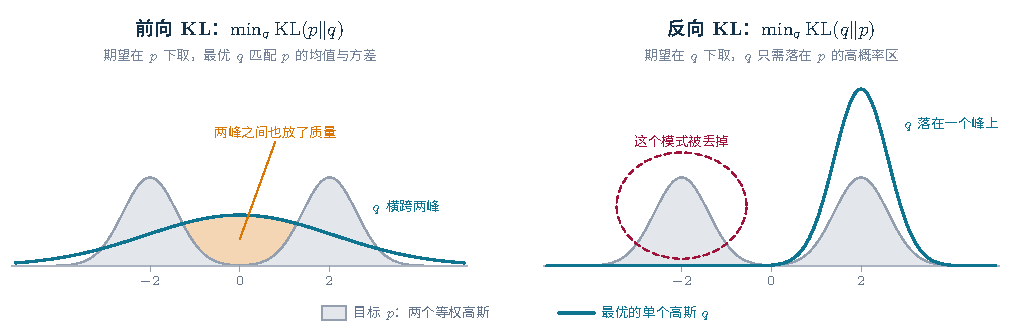
\includegraphics[width=\textwidth]{kl_direction.pdf}
\caption{用单个高斯 \(q\) 拟合双峰目标 \(p\) 时，KL 的两个方向给出不同的最优解。左：前向 \(\KL(p\Vert q)\) 的最优 \(q\) 与 \(p\) 同均值、同方差，覆盖两个模式，同时在两峰之间放了 \(p\) 几乎没有的质量（橙色）。右：反向 \(\KL(q\Vert p)\) 的最优 \(q\) 近似贴合一个峰，丢掉另一个模式；按对称性，落在左峰同样最优。}
\label{fig:kl-direction}
\end{figure}

\subsection{玻尔兹曼分布与变分自由能}
\label{sec:free-energy}

对玻尔兹曼目标 \(\pi(x)=Z^{-1}\exp[-\beta E(x)]\)，任意归一化试探分布 \(q_\theta\) 满足（其中 \(\beta=1/(k_BT)\)，\(T\) 为温度，\(k_B\) 为玻尔兹曼常数）
\begin{align}
 \KL(q_\theta\Vert\pi)&=\E_{q_\theta}[\log q_\theta(x)+\beta E(x)]+\log Z,\\
 F[q_\theta]&=\E_{q_\theta}[E(x)]-T S[q_\theta],\qquad S[q]=-k_B\E_q[\log q].
\end{align}
所以最小化变分自由能等价于最小化 \(\KL(q_\theta\Vert\pi)\)。这条关系将统计物理中的低能量、高熵平衡与生成模型中的样本质量、分布覆盖联系起来。

\begin{figure}[H]
\centering
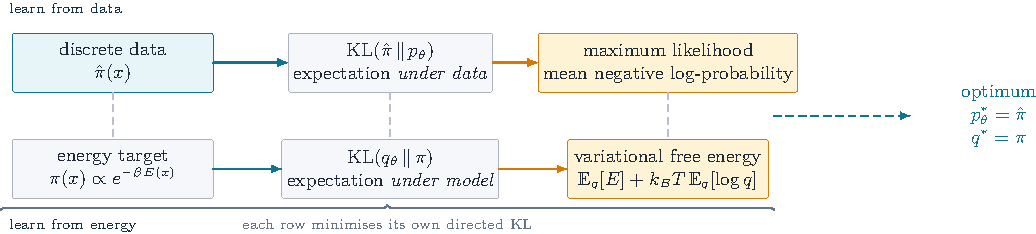
\includegraphics[width=\textwidth]{mle_free_energy.pdf}
\caption{两个方向的 KL 对应不同的学习目标。上行从离散数据学习分布，下行从已知能量学习平衡分布；前者导出下一章的最大似然，后者导出变分自由能。在不限制模型表达能力时，两者各自以匹配其目标分布为最优解。}
\label{fig:mle-free-energy}
\end{figure}

\subsection{从抽样分布看训练梯度}
\label{sec:gradient-estimator-map}

后面几类模型的训练目标都会出现同一步：从一个含参数 \(q_\eta\) 的分布里抽样，再对样本上的目标求期望。先把两条求导路径放在一起，遇到具体模型时可以直接对照；第 \ref{chap:model-families} 章变分自编码器（Variational Autoencoder，VAE）的连续潜变量走重参数化，第 \ref{chap:training-methods} 章的策略梯度走 score-function。

图 \ref{fig:mle-free-energy} 的两行还提示了训练梯度的区别。若样本来自固定的经验分布，且 \(\log p_\theta(x)\) 可以直接求值，最大似然损失满足 \(\nabla_\theta[-\E_{\hat\pi}\log p_\theta(x)]=-\E_{\hat\pi}\nabla_\theta\log p_\theta(x)\)：对每个真实样本直接反向传播即可。若目标包含 \(J(\eta)=\E_{u\sim q_\eta}[h_\eta(u)]\)，而该期望需要从依赖 \(\eta\) 的分布抽样估计，就必须处理参数如何影响被抽到的 \(u\)。两种常用路径是
\begin{align}
 \nabla_\eta J
 &=\E_{q_\eta}\!\left[\nabla_\eta h_\eta(u)
 +(h_\eta(u)-b)\nabla_\eta\log q_\eta(u)\right],
 &&\text{score-function},\\
 \nabla_\eta J
 &=\E_{\epsilon\sim p(\epsilon)}\!\left[
 \frac{d}{d\eta}h_\eta(g_\eta(\epsilon))\right],
 \quad u=g_\eta(\epsilon),
 &&\text{重参数化}.
\end{align}
这里 \(b\) 不依赖当前抽到的 \(u\)，可作为 baseline 降低第一种估计的方差~\cite{zhang2023admc}；第二种写法把随机性移到与 \(\eta\) 无关的 \(\epsilon\)，再沿确定性的 \(g_\eta\) 使用链式法则。两式都保留了 \(h_\eta\) 本身对参数的直接导数。强化学习大量使用第一条路径：策略从 \(\pi_\theta\) 抽取动作或整条轨迹，以回报乘以 \(\nabla_\theta\log\pi_\theta\) 构造蒙特卡洛策略梯度；后文的近端策略优化（Proximal Policy Optimization，PPO）和组相对策略优化（Group Relative Policy Optimization，GRPO）用优势替代原始回报，并加入概率比、裁剪等机制。

\begin{table}[H]
\centering\small
\begin{tabularx}{\textwidth}{>{\bfseries}p{28mm} X X X}
\toprule
梯度路径 & 适用条件 & 梯度从哪里来 & 优势与代价\\
\midrule
Score-function & 可计算并求导 \(\log q_\eta(u)\)；\(u\) 可离散，参数无关的 \(h\) 可为黑盒 & 目标值乘以 \(\nabla_\eta\log q_\eta(u)\) & 适用面广；方差通常较高，常配合 baseline\\
重参数化 & 可写成可微的 \(u=g_\eta(\epsilon)\)，且后续目标对 \(u\) 可微 & 沿 \(h_\eta\) 与 \(g_\eta\) 的计算图回传 & 利用样本方向上的导数，方差通常较低；需要可微路径\\
\bottomrule
\end{tabularx}
\caption{从参数化抽样分布求训练梯度的两条路径。}
\label{tab:gradient-estimator-map}
\end{table}

下文读到新的训练目标时，可先看抽样分布是否含待优化参数，再用表 \ref{tab:gradient-estimator-map} 判断梯度怎样通过采样步骤。VAE 的连续潜变量和 GAN 的连续生成路径使用重参数化一侧的路径梯度；从模型采样离散 token、自旋或线路结构并按评分更新其分布时，常用 score-function。
